\subsection{Recap: How to Implement Features?}
\begin{frame}{\myframetitle}
	\begin{mycolumns}
		\myexampletight{Given a feature model for graphs \ldots}{
			\centering\featureDiagramGraphs
			%\featureDiagramLegend
		}
		\myexample{\ldots\ we can derive a valid configuration}{
			\small
			\leftmiddleandright{
				$\{G\}$\\
				$\{G,C\}$\\
				$\{G,D\}$\\
				$\{G,C,D\}$\\
			}{
				$\{G,W\}$\\
				$\{G,C,W\}$\\
				$\{G,D,W\}$\\
				$\{G,C,D,W\}$\\
			}{
				$\{G,W,S\}$\\
				$\{G,C,W,S\}$\\
				$\{G,D,W,S\}$\\
				$\{G,C,D,W,S\}$\\
			}
		}
	\mynextcolumn
		\vspace{-10mm}
		\myexampletight{How to Generate Products Automatically?}{
			\centering\foreach \page in {2,12,4,14,6,16,8,18,10,20,42,44}{\includegraphics[width=.23\linewidth,page=\page]{graphs} }
		}
		\mynote{Goals}{
			\begin{itemize}
				\item Descriptive specification of a product (i.e., a configuration, a selection of features)
				\item Automated generation of a product with compile-time variability
			\end{itemize}			
		}
	\end{mycolumns}
\end{frame}

\begin{frame}{Recap: Features with Build Systems}
	\begin{mycolumns}[widths={40,60},animation=none]
		\myexampletight{}{
			\centering
			\pic[width=.65\linewidth]{pignap-features}
		}
	\mynextcolumn
		\mydefinition{Conditional Compilation with Build Systems}{
			\begin{itemize}
				\item Exploit the expressiveness of a build system's configuration language
				\item In- and exclude individual files or entire directories based on feature selection
			\end{itemize}
		}
		\uncover<2->{\mynote{Major Challenges}{
			\begin{itemize}
				\item Build scripts may become complex, there is no limit to what can be done (e.g., you can run arbitrary shell commands on files)\\
					$\Rightarrow$ \emph{Hard to understand and analyze}
				\item No simple in- and exclusion of individual lines or chunks of code\\
					$\Rightarrow$ High-level use \emph{only}!
			\end{itemize}
		}}
	\end{mycolumns}
\end{frame}

\begin{frame}{Recap: Features with Preprocessors}
	\begin{mycolumns}[widths={40,60},animation=none]
		\myexampletight{}{
			\centering
			\pic[width=\linewidth,page=1,trim=15 20 185 40,clip]{preprocessor-wilderness}
		}
	\mynextcolumn
		\mydefinition{Conditional Compilation with Preprocessors}{
			\begin{itemize}
				\item Use conditional compilation facilities provided by preprocessors 
				\item Annotate and potentially remove code fragments, depending on feature selection
			\end{itemize}
		}
		\uncover<2->{\mynote{Major Challenges}{
			\begin{itemize}
				\item May \emph{obfuscate} source code and severely impact its readability
				\item Hard to analyze and process for existing IDEs
				\item Often used in an ad-hoc or \emph{undisciplined} fashion
				\item Prone to subtle syntax, type, or runtime errors which are hard to detect
				\item \emph{Scattering} and \emph{tangling}\\
				$\Rightarrow$ separation of concerns?
			\end{itemize}
		}}
	\end{mycolumns}
\end{frame}


\subsection{Recap: UML Component Diagram}
\subsection{Vision: Component Markets}
\subsection{The Library Scaling Problem}
\subsection{Components in Java}
\subsection{Components for Features}
\subsection{Discussion}

